Our initial idea was to simply create node on each walkable square in the grid to be a node as illustrated in \ref{gridGraph}.
A node would then have up to eight connections which would point to a neighbour of that certain node with a cost of traversing to this node.
Possible neighbours would be four to each side of the node with a cost of 10 and four diagonal neighbours with a cost of 14, which is the length of the hypotenuse when the length of the catheti are 10.
\begin{figure}[H]
	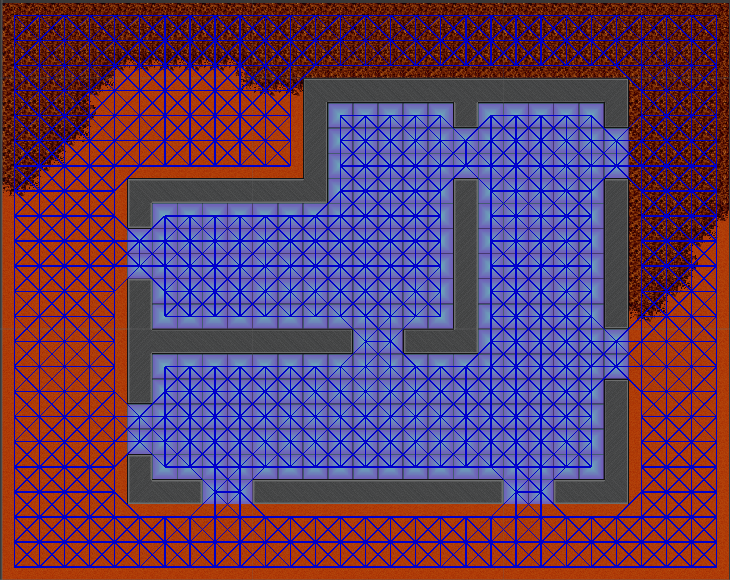
\includegraphics[width=\textwidth]{figures/astar/gridGraph}
	\caption{Graph based on the grid of the map}
	\label{gridGraph}
\end{figure}

To navigate in the graph a pathfinding algorithm is needed. 
The pathfinding algorithm that will be used is A* search pathfinding which has a runtime of $O(n \times m)$, where n is the number of nodes that will be explored, m is the average number of neighbours in the graph, and it is assumed that the graph and heuristic operations take constant time \cite{AIG:Millington}.

\subsection*{Choosing a heuristic}
The heuristic should be easily calculated and somewhat precise since it should be called on runtime.
It is desired to have an heuristic which underestimates since overestimating can result in an incorrect shortest-path.
When working with grid maps three different heuristics are commonly used: % http://theory.stanford.edu/~amitp/GameProgramming/Heuristics.html
\begin{itemize}
\item Manhattan Distance
\item Chebyshev Distance
\item Euclidean Distance
\end{itemize}
The Manhattan distance works very well on grid based maps. 
It is a simple heuristic, it works by adding the distance between the current node's x-coordinate and the goal node's x-coordinate, and the distance between the current node's y-coordinate and the goal node's y-coordinate.
However, it does not support diagonal movement. 
This means the heuristic will have a tendency to overestimate which will make it non-admissible heuristic.\\\\
The Chebyshev distance works almost in the same way, however, this heuristic take diagonal movement into account. 
It assumes that diagonal cost is equal to the side costs, this results in an underestimation or an exact cost of the path.\\\\
The last heuristic uses the euclidean distance between the current node and the goal node as the heuristic.
This however is more expensive to calculate.\\\\
Looking at these heuristics we find that the best prospect for our heuristic will be Chebyshev since it is faster than euclidean but also works with diagonal movement.

This approach resulted in a very large graph which took a lot of time to create and traverse through, when running the algorithm on it.
An example of this can be seen in figure \ref{gridGraph} where you can see a map of size 64x64, the graph created for that map has 3984 nodes and 30450 edges.